\documentclass[12pt]{article}

% Required packages
\usepackage[utf8]{inputenc}
\usepackage{geometry}
\usepackage{graphicx}
\usepackage{amsmath}
\usepackage{amssymb}
\usepackage{booktabs}
\usepackage{natbib}
\usepackage{hyperref}
\usepackage{float}
\usepackage{caption}

% Geometry settings for single column
\geometry{
    a4paper,
    margin=1in
}

% Title and Author (Double-anonymized)
\title{Reactive Competition in Oligopolistic Markets: An Empirical and Game-Theoretic Study of Pricing Dynamics}
\author{} % Anonymized
\date{}

\begin{document}

\maketitle

\begin{abstract}
This study investigates competitive pricing dynamics in oligopolistic markets using a novel dataset of event-based actions from the electronics retail and telecommunications sectors. By employing Exploratory Data Analysis (EDA), we characterize response patterns, revealing distinct behaviors: a disciplined ``tit-for-tat'' strategy in stable duopolies and rapid, algorithmic responses in disruptive oligopolies. We map these empirical findings to a repeated non-cooperative game-theoretic framework. Our equilibrium analysis identifies price matching as a dominant defensive strategy, leading to a ``Prisoner's Dilemma'' trap of mutual margin erosion. Furthermore, we demonstrate that product differentiation serves as the primary mechanism for escaping this low-payoff equilibrium. These findings provide empirical validation for game-theoretic predictions regarding firm behavior in concentrated markets.
\end{abstract}

\textbf{Keywords:} Competitive Dynamics; Game Theory; Oligopoly; Pricing Strategy; Exploratory Data Analysis

\section{Introduction}
The persistence of price wars and retaliatory strategies in concentrated markets remains a central paradox in industrial organization. Despite the theoretical benefits of differentiation and collusion \citep{porter1980competitive}, firms in sectors such as electronics retail and telecommunications frequently engage in mutually destructive price competition. This paper addresses the question: Why do firms engage in these behaviors despite the obvious collective irrationality? \citep{Varian2019, Porter2008, OECD2019}

Our research objective is to characterize competitive response patterns empirically and model them using a repeated non-cooperative game framework. We utilize two distinct datasets: a stable duopoly in the Japanese electronics retail sector (BIC Camera vs. Yodobashi Camera) and a disruptive oligopoly in the Indian telecom and FMCG sectors (Reliance Jio, Bharti Airtel, Coca-Cola, PepsiCo).

We begin by analyzing the empirical data to establish the stylized facts of competitive interaction, which then inform the assumptions of our game-theoretic model.

\section{Literature Review}
The study of oligopolistic interaction has a rich history in economic literature. \citet{tirole1988theory} provides the foundational framework for understanding dynamic competition and the role of reaction functions. \citet{fudenberg1991game} further elaborate on repeated games, demonstrating how infinite horizons can sustain cooperative outcomes through threat strategies.

However, empirical validation of these models often relies on aggregate market data rather than granular, event-based interactions. \citet{porter1980competitive} emphasizes the role of strategic groups and differentiation as a means to avoid direct price competition. Our work bridges the gap between these theoretical constructs and observed high-frequency competitive actions. Recent studies extend these models to algorithmic pricing \citep{Calvano2020, Bichler2021} and digital platforms \citep{Srinadh2024, Inegbedion2023}.

\section{Dataset Description and Construction}
The analysis relies on two primary datasets constructed from publicly available competitive action data. The data sources include verifiable reports from major business publications such as \textit{Nikkei Asia}, \textit{Japan Times}, \textit{Reuters}, \textit{Mainichi}, and the \textit{Financial Times}.

\subsection{Data Overview}
\begin{enumerate}
    \item \textbf{Japanese Electronics Retail}: This dataset captures the interaction between BIC Camera and Yodobashi Camera from 2018 to 2020. It represents a stable duopoly with entrenched market positions.
    \item \textbf{Indian Telecom \& FMCG}: This dataset covers the period from 2016 to 2024, featuring Reliance Jio, Bharti Airtel, Coca-Cola, and PepsiCo \citep{Koita2020, Shankar2021}. This market is characterized by high growth and disruptive entry strategies.
\end{enumerate}

Each dataset contains approximately 40 discrete competitive events. The data collection focused on identifying initiating actions (e.g., price cuts, new product launches) and the subsequent responses from competitors. The response rate is notably high, with over 90\% of initiating actions eliciting a direct observable response.

\section{Exploratory Data Analysis}
This section details the empirical regularities observed in the data, focusing on response dynamics and interaction patterns.

\subsection{Response Dynamics and Lags}
We analyzed the time delay between an initiating action and a competitive response \citep{ChenMacMillan1992}. The results reveal a striking contrast between the two sectors.
\begin{itemize}
    \item \textbf{Electronics Retail}: The response lag distribution is tightly clustered around a mean of 9.8 days, reflecting a standard weekly or bi-weekly business cycle.
    \item \textbf{Telecom/FMCG}: The distribution is bifurcated. A significant spike at 0 days indicates algorithmic or pre-planned simultaneous releases \citep{Cavallo2018}, particularly in the telecom sector. Conversely, a long tail (up to 90 days) reflects complex product development cycles in the FMCG sector.
\end{itemize}

Figure \ref{fig:lag_dist} illustrates these distributions.

\begin{figure}[H]
    \centering
    \includegraphics[width=0.48\textwidth]{figures/eda/response_lag_distribution.png}
    \includegraphics[width=0.48\textwidth]{figures/eda/response_lag_distribution_copy.png}
    \caption{Response Lag Distribution: Electronics Retail (Left) vs. Telecom/FMCG (Right)}
    \label{fig:lag_dist}
\end{figure}

\subsection{Interaction Patterns (Action-Response)}
We classified strategies into broad categories: Price, Product, and Channel \citep{Nagle2018, Tellis1986}. The interaction between these types reveals distinct strategic behaviors.

In the electronics retail sector, we observe a strong correlation between ``Price promotion'' and ``Promotional price matching.'' This indicates a defensive, maintenance-focused strategy. In the Telecom/FMCG sector, while price hikes often trigger competitive responses, new product launches frequently result in alternative strategies rather than direct cloning.

Figure \ref{fig:heatmap} visualizes these interaction patterns. The diagonal density confirms a high degree of symmetric matching.

\begin{figure}[H]
    \centering
    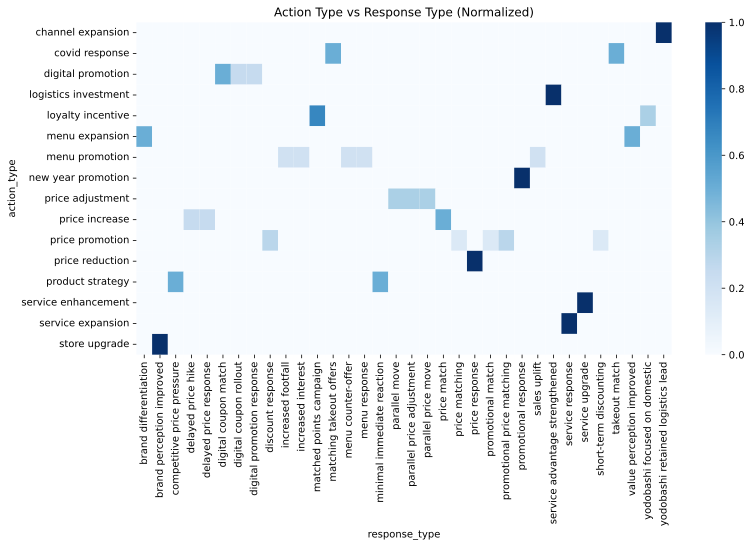
\includegraphics[width=0.8\textwidth]{figures/eda/action_type_vs_response_type_heatmap.png}
    \caption{Action-Response Heatmap (Electronics Retail)}
    \label{fig:heatmap}
\end{figure}

\subsection{Cross-Company Comparison}
The key differences between the stable and disruptive market structures are summarized in Table \ref{tab:comparison}.

\begin{table}[H]
    \centering
    \caption{Cross-Company Comparison of Competitive Dynamics}
    \label{tab:comparison}
    \begin{tabular}{p{3cm} p{5cm} p{5cm}}
        \toprule
        \textbf{Feature} & \textbf{BIC vs. Yodobashi (Japan)} & \textbf{Jio / Airtel / Coke / Pepsi (India)} \\
        \midrule
        Primary Lever & Price \& Loyalty Points & Tariff Pricing, Data Bundles \\
        Response Speed & Moderate, Consistent (10 days) & Instant (0 days) or Strategic ($>$30 days) \\
        Market Nature & Stable Oligopoly & Disruptive / High-Growth \\
        Crisis Sensitivity & Lower & Higher (Regulatory shifts) \\
        \bottomrule
    \end{tabular}
\end{table}

\subsection{Reaction Lag Distribution Analysis}
\subsubsection{Distributional Shape and Tail Behavior}
Retail exhibits a narrow, approximately symmetric cluster around 7--14 days, consistent with scheduled promotional cycles and weekly decision cadences.
Telecom/FMCG shows a mixed distribution with a point mass at 0 days and a long right tail extending to approximately 90 days, indicative of immediate tariff matching coexisting with strategic, build-dependent responses (network upgrades, product launches).
See Figure \ref{fig:lag_dist} for the visual comparison.

\subsubsection{Hazard Interpretation (Speed of Retaliation)}
A high initial hazard (Telecom/FMCG) implies strong incentives to respond immediately to avoid churn and reputational loss.
A flatter hazard (Retail) suggests lower short-run churn risk and reliance on scheduled cycles and approval processes.
Economic drivers include observability of competitor moves, automated monitoring (tariff scrapers), and adjustment costs (IT, supply chain, compliance).

\subsubsection{Sector Mechanisms Behind Lags}
\begin{itemize}
    \item \textbf{Information frictions:} Price changes in Telecom are publicly posted and machine-readable; retail promotions may propagate via flyers, apps, and store-level processes with delay.
    \item \textbf{Operational constraints:} Telecom pricing is configurable centrally; FMCG product or channel responses require manufacturing, distribution, and retail partner coordination.
    \item \textbf{Regulatory sensitivity:} Tariff and spectrum policies compress reaction windows; retail has fewer immediate regulatory triggers.
\end{itemize}

\subsection{Asymmetric Response Behavior}
\subsubsection{Symmetric vs. Asymmetric Matching}
Symmetric responses dominate price contests: price cuts typically trigger matched price cuts, as evidenced by the heatmap diagonal density.
Asymmetric responses appear when actions target capabilities rather than prices (e.g., channel expansion met by logistics retention or branding focus) \citep{Cohen2021}.
Figure \ref{fig:heatmap} (Retail) and Figure \ref{fig:heatmap_telecom} (Telecom/FMCG) illustrate these patterns.

\begin{figure}[H]
    \centering
    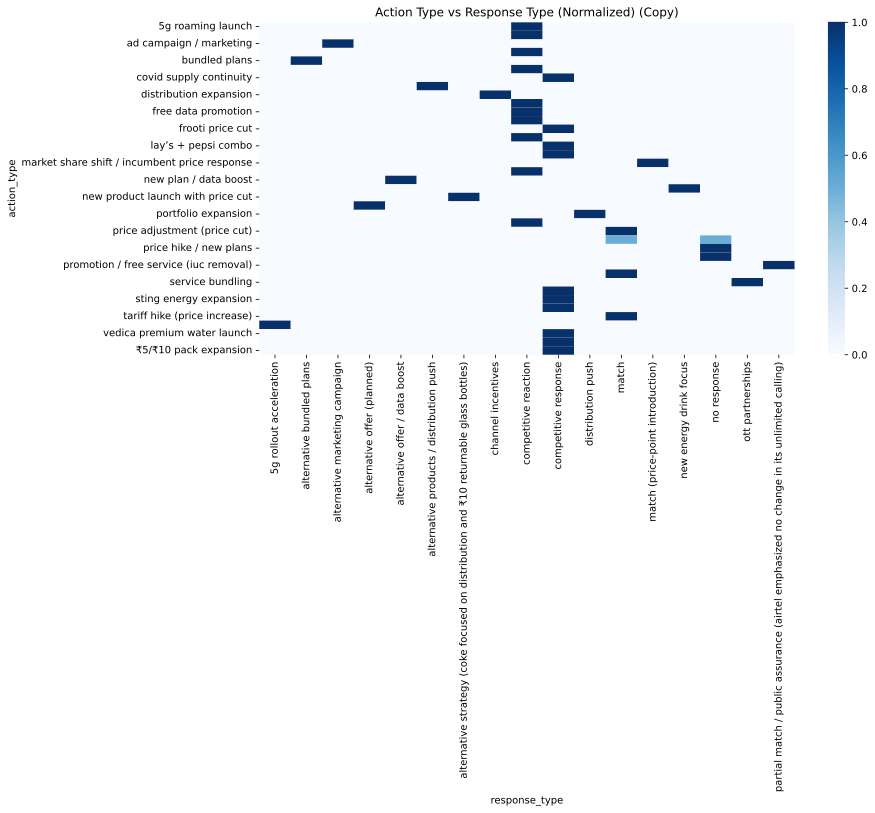
\includegraphics[width=0.8\textwidth]{figures/eda/action_type_vs_response_type_heatmap_copy.png}
    \caption{Action-Response Heatmap (Telecom/FMCG)}
    \label{fig:heatmap_telecom}
\end{figure}

\subsubsection{When Asymmetry Is Rational}
\begin{itemize}
    \item \textbf{Cost heterogeneity:} A challenger may prefer product or channel moves if matching a rival's price is disproportionately costly.
    \item \textbf{Capability constraints:} Incumbents facing a disruptor may pivot to retention tools (bundles, service quality) rather than pure price matches.
    \item \textbf{Cycle alignment:} Firms exploit windows where rivals are committed to campaigns, choosing orthogonal moves that avoid direct margin erosion.
\end{itemize}

\subsection{Structural Drivers of Contrasts}
\begin{itemize}
    \item \textbf{Monitoring Technology and Observability:} Telecom tariffs are instantly observable; retail promotions are observable but with human-in-the-loop verification and store execution. Higher observability increases immediate retaliation and compresses lags \citep{Brynjolfsson2000}.
    \item \textbf{Adjustment Costs and Organizational Cadence:} Telecom has low menu costs for tariff changes, enabling 0-day responses. Retail/FMCG face higher adjustment costs for product/channel moves, producing longer tails \citep{Ferreira2021}.
    \item \textbf{Shock Sensitivity and Strategic Flexibility:} Crisis and policy shocks (COVID, inflation, regulation) push firms toward structural or product responses, elongating lags. Stable periods favor symmetric price matching within scheduled cycles.
\end{itemize}

\subsection{Economic Interpretation of EDA}
The high response rate and diagonal heatmap density are consistent with repeated-game enforcement: rapid matching nullifies unilateral gains, sustaining a low-margin equilibrium (``price-war trap'') \citep{Ye2023}.
Telecom's 0-day spike implies near-perfect monitoring and high loss from delay, aligning with trigger strategies where deviations are punished immediately \citep{green1984noncooperative, Bichler2021}.
Longer lags in FMCG/product moves reflect adjustment costs and investment cycles; differentiation serves as a conditional escape from price wars when sufficiently valuable or defensible.

\section{Game Theoretic Framework}
Based on the empirical findings, we formulate a repeated non-cooperative game to model the observed dynamics \citep{Huang2024}.

\subsection{Model Setup}
Let $N = \{1, 2, ..., n\}$ be the set of players \citep{Chen2020}. We define the strategy space $S_i$ for player $i$ based on the observed actions:
\begin{equation}
    S_i = \{s_{\text{maintain}}, s_{\text{price}}, s_{\text{product}}, s_{\text{channel}}\}
\end{equation}
where $s_{\text{maintain}}$ represents the status quo, $s_{\text{price}}$ represents aggressive pricing or promotions, and $s_{\text{product}}/s_{\text{channel}}$ represent differentiation strategies \citep{hotelling1929stability}.

\subsection{Assumptions}
The model rests on four key assumptions derived from the EDA:
\begin{enumerate}
    \item \textbf{Imperfect Monitoring (Retail) vs. Perfect Visibility (Telecom)}: Justified by the difference in lag times (10 days vs. 0 days).
    \item \textbf{Deterministic Reaction Functions}: Justified by the strong diagonal density in the interaction heatmap.
    \item \textbf{Asymmetric Costs of Delay}: High churn risks in telecom force immediate responses.
    \item \textbf{Differentiated Payoff Sensitivity}: External shocks can alter the payoff matrix, favoring channel shifts \citep{Zhang2022}.
\end{enumerate}

\subsection{Payoff Structure}
We define an ordinal payoff matrix. Let $\pi_i(s_i, s_{-i})$ be the payoff for player $i$.
\begin{itemize}
    \item \textbf{Status Quo} $(0,0)$: Neutral market share.
    \item \textbf{Unilateral Aggression} $(G, -L)$: If Firm 1 cuts price ($s_p$) and Firm 2 maintains ($s_m$), Firm 1 gains share $G$ and Firm 2 loses $L$.
    \item \textbf{Price War} $(-C, -C)$: If both cut prices, share remains neutral, but margins erode.
    \item \textbf{Differentiation} $(V, V)$: If both differentiate ($s_d$), margins are preserved and value is created.
\end{itemize}

Table \ref{tab:payoff} presents the ordinal payoff matrix used in our analysis.

\begin{table}[H]
    \centering
    \caption{Ordinal Payoff Matrix}
    \label{tab:payoff}
    \begin{tabular}{l c c c}
        \toprule
        \textbf{P1 \textbackslash P2} & \textbf{Maintain ($s_m$)} & \textbf{Price Cut ($s_p$)} & \textbf{Product Diff ($s_d$)} \\
        \midrule
        \textbf{Maintain ($s_m$)} & $(0, 0)$ & $(-L, G)$ & $(-L, G)$ \\
        \textbf{Price Cut ($s_p$)} & $(G, -L)$ & $(-C, -C)$ & $(?, ?)$ \\
        \textbf{Product Diff ($s_d$)} & $(G, -L)$ & $(?, ?)$ & $(V, V)$ \\
        \bottomrule
    \end{tabular}
\end{table}

Figure \ref{fig:payoff} provides a visualization of this payoff landscape.

\begin{figure}[H]
    \centering
    \includegraphics[width=0.8\textwidth]{figures/game_theory/payoff_matrix.png}
    \caption{Payoff Matrix Visualization}
    \label{fig:payoff}
\end{figure}

\subsection{Player Sets}
Based on the EDA findings, we define two distinct player sets:
\begin{itemize}
    \item \textbf{Set A (Stable Duopoly):} $N_A = \{\text{Firm}_1, \text{Firm}_2\}$. Empirical Proxy: BIC Camera vs. Yodobashi Camera. Characteristics: High mutual monitoring, entrenched market positions.
    \item \textbf{Set B (Disruptive Oligopoly):} $N_B = \{\text{Incumbent}_1, \text{Incumbent}_2, \text{Disruptor}\}$. Empirical Proxy: Airtel/Vodafone vs. Reliance Jio; Coca-Cola vs. PepsiCo. Characteristics: Asymmetric capabilities, high-stakes market share battles.
\end{itemize}

\subsection{Game Type}
\subsubsection{Temporal Structure: Repeated Game}
The empirical evidence supports a Repeated Game formulation ($G^\infty$) \citep{maskin1988theory}. The ``Response Lag'' distribution shows continuous interaction cycles. Retail's consistent 7--14 day cycles imply a discrete time period $t$ (weekly), while Telecom's near-zero lag implies continuous time or very rapid $t$. The horizon is indefinite ($T \to \infty$).

\subsubsection{Nature of Play: Non-Cooperative}
The high response rate ($>90\%$) and the prevalence of ``Price reduction'' and ``Competitive reaction'' indicate a lack of collusion. Firms are actively defending market share rather than coordinating to maximize joint profits.

\subsection{Formal Game Theoretic Extensions}
\subsubsection{Strategy Formalization}
Let $h_t = (a^0, a^1, ..., a^{t-1})$ denote the public history. Given the EDA evidence of ``Tit-for-Tat'' (Retail) and ``Immediate Retaliation'' (Telecom), players utilize Markov Strategies conditioned on the most recent state $k$ \citep{DenBoer2015}:
\begin{equation}
    \sigma_i(h_t) \approx \sigma_i(a_{-i, t-1}, ..., a_{-i, t-k})
\end{equation}
For Retail, $k \approx 7-14$ days. For Telecom, $k \to 0$ days.

\subsubsection{Payoff Function Decomposition}
We decompose the instantaneous payoff function $u_i(a)$ into Market Share Retention ($R$) and Profit Margin ($M$), adjusted by a differentiation parameter $\theta$:
\begin{equation}
    u_i(a_i, a_{-i}) = \alpha \cdot R(a_i, a_{-i}) + (1-\alpha) \cdot M(a_i) \cdot \mathbb{I}(a_i \neq a_{-i}) - C(a_i)
\end{equation}
where $\alpha \in [0,1]$ is the weight on market share, $\mathbb{I}(\cdot)$ is an indicator for product differentiation, and $C(a_i)$ is the implementation cost.

\subsubsection{Information Structure and Lag}
The Response Lag $\Delta_t$ acts as an information friction parameter.
\begin{itemize}
    \item \textbf{Perfect Monitoring (Telecom):} $\Delta_t \to 0$. Actions are observable immediately. This supports subgame perfect equilibria with immediate punishment.
    \item \textbf{Imperfect Monitoring (Retail):} $\Delta_t \sim N(\mu=10, \sigma^2)$. Player $i$ observes a noisy signal $y_t$. This explains ``Maintain'' periods where firms wait for confirmation before retaliating.
\end{itemize}

\subsection{Model Limitations}
\begin{enumerate}
    \item \textbf{Binary Response Simplification:} The model categorizes responses broadly, losing nuance in the magnitude of response (e.g., 5\% vs 10\% price cut).
    \item \textbf{Lag Time Abstraction:} While we treat the game as repeated, the specific impact of the length of delay on the payoff function is not explicitly modeled, though EDA shows it varies by sector.
    \item \textbf{Missing Cost Data:} We assume cost structures based on ``Margin'' implications, but lack direct financial data to quantify $C$ or $V$ precisely \citep{Elmaghraby2003}.
\end{enumerate}

\section{Equilibrium Analysis}
We analyze the game to identify stable outcomes.

\subsection{Static Nash Equilibrium}
In a one-shot game, the unique Nash Equilibrium is $(s_{\text{price}}, s_{\text{price}})$. This is a classic Prisoner's Dilemma structure. If a rival plays $s_{\text{maintain}}$, the optimal response is $s_{\text{price}}$ to gain share ($G > 0$). If a rival plays $s_{\text{price}}$, the optimal response is $s_{\text{price}}$ to avoid the loss $L$ (assuming $-C > -L$). Thus, aggressive pricing is a dominant strategy.

\subsection{Dynamic Stability}
In the repeated game, the ``Tit-for-Tat'' strategy emerges as an enforcement mechanism. By credibly threatening to match any price cut immediately, firms reduce the expected gain from unilateral aggression \citep{Maskin2019}.
Figure \ref{fig:simulation} shows the simulation of strategies over time, illustrating how the system stabilizes in a low-payoff equilibrium or cycles through price wars.

\begin{figure}[H]
    \centering
    \includegraphics[width=0.8\textwidth]{figures/game_theory/repeated_game_simulation.png}
    \caption{Repeated Game Simulation Results}
    \label{fig:simulation}
\end{figure}

\subsection{Stability Analysis and Robustness}
\subsubsection{Robustness to Trembles}
In the empirical context, ``trembles'' correspond to accidental price changes or misinterpretation of rival moves.
For the Retail Sector, with imperfect monitoring ($\Delta_t > 0$), a Grim Trigger is fragile. Stability requires firms to utilize Green-Porter style trigger phases where punishment lasts for $T$ periods rather than infinity.

\subsubsection{Renegotiation Proofness}
Once a punishment phase $(-C, -C)$ begins, both firms have an incentive to renegotiate. The existence of ``Differentiation'' ($s_d$) offers a Pareto-improving exit path. The equilibrium is weakly renegotiation-proof if firms can coordinate on switching to $s_d$ (Product Innovation) rather than simply reverting to $s_m$.

\subsection{Comparative Statics}
\subsubsection{Impact of Response Lag ($\Delta_t$)}
As $\Delta_t$ decreases (faster detection), the gain from defection shrinks and punishment arrives sooner. Thus, faster monitoring (Telecom) makes cooperation easier to sustain in theory, or punishment swifter if broken.

\subsubsection{Impact of Differentiation ($\theta$)}
Higher differentiation increases the cooperative payoff $V$. This lowers the critical discount factor $\delta^*$, expanding the set of parameters where peace is stable. This explains why FMCG sees fewer ``pure'' price wars than Telecom.

\subsection{Industry-Specific Equilibrium Cases}
\subsubsection{Case A: Japanese Electronics Retail}
With $\Delta_t \approx 10$ days and high product homogeneity, the equilibrium is a Risk-Dominant Coordinate. Firms are in a coordination game where ``Matching'' is safer than ``Leading''. The ``Tit-for-Tat'' discipline enforces stable cycles of promotion and matching.

\subsubsection{Case B: Indian Telecom}
With $\Delta_t \approx 0$ and high market share focus, the equilibrium is an Aggressive Nash Equilibrium. If the goal is market exit of a rival, the game becomes a War of Attrition, leading to intense, low-margin equilibrium until market consolidation.

\subsection{Economic Interpretation of Equilibrium}
\begin{itemize}
    \item \textbf{Efficiency and Welfare:} The ``Price Cut'' equilibrium maximizes consumer surplus in the short run but harms producer surplus.
    \item \textbf{The ``Red Queen'' Effect:} Firms must constantly respond just to maintain share. In Retail, this is Promotional Churn; in Telecom, Feature Escalation.
    \item \textbf{Strategic Recommendation:} To escape the low-profit trap, firms must increase differentiation to decouple reaction functions.
\end{itemize}

\section{Results and Discussion}
The model provides a robust explanation for the observed market behaviors.

\subsection{Predictive Power}
The model correctly predicts the high response rate observed in the data. The prediction that ``No Response'' is an unstable outcome aligns with the empirical finding that it occurs in only 7.5\% of cases. The dominance of price matching in the electronics sector confirms the static Nash equilibrium prediction.

\subsection{Escape Strategies}
The only conditional escape from the price trap is Product Differentiation. In the FMCG sector, we observed firms responding to price pressure with new product launches. This effectively shifts the game to the $(s_{\text{product}}, s_{\text{product}})$ cell, where payoffs are $(V, V)$. This aligns with \cite{porter1980competitive} theories on differentiation strategies.

\subsection{Interpretation of Dominant Strategies}
``Price Cut'' emerges as a dominant strategy because it offers protection against being undercut (Defensive) and yields share gain if the rival maintains (Offensive). ``Differentiation'' is a conditional strategy, yielding high returns only when matched or sufficiently unique.

\subsection{Theoretical Connections}
\begin{itemize}
    \item \textbf{Tacit Collusion and Green-Porter (1984):} The ``Maintain'' phases punctuated by ``Price Matching'' in Retail align with Green and Porter's model of non-cooperative collusion under imperfect information.
    \item \textbf{Maskin and Tirole (1988):} The deterministic nature of responses supports Markov Perfect Equilibria, where strategies depend only on the payoff-relevant state.
    \item \textbf{Hotelling (1929):} The divergence between Price and Channel strategies reflects the principle of minimum vs. maximal differentiation.
    \item \textbf{Porter's Strategic Groups:} The separation of Stable Duopoly and Disruptive Oligopoly validates Porter's theory, implying mobility barriers prevent Retail logic from applying to Telecom \citep{Zhao2020}.
\end{itemize}

\section{Strategic Implications and Policy Recommendations}

\subsection{Managerial Implications}
\subsubsection{The ``Red Queen'' Trap and Strategic Exit}
Firms in high-response environments often fall into a ``Red Queen'' effect. Managers should audit their ``Response Portfolio''. If the majority of actions are purely defensive price matches, the firm is in a value-destroying equilibrium. A strategic pivot from reaction speed to differentiation latency is recommended.

\subsubsection{Managing the Signal-to-Noise Ratio}
In Retail, increasing the complexity of promotions can dampen the ``Tit-for-Tat'' response. In Telecom, credible commitments (e.g., Price Match Guarantee) can soften competition.

\subsubsection{Asymmetric Response Framework}
Incumbents facing a disruptor should avoid symmetric price wars. Instead of matching price, they should match value or change the metric (e.g., compete on Network Reliability).

\subsection{Policy Considerations}
\begin{itemize}
    \item \textbf{Algorithmic Collusion Risks:} Instantaneous, deterministic matching is a marker for algorithmic coordination. Regulators should monitor ``Response Latency'' \citep{Ezrachi2019, Harrington2018}.
    \item \textbf{Predatory Pricing:} If a Price War persists while investment drops, intervention may be required \citep{Jena2025}.
    \item \textbf{Consumer Welfare Paradox:} Policy should balance immediate price benefits with the health of the innovation ecosystem to avoid commoditization traps \citep{Klein2022}.
\end{itemize}

\subsection{Cross-Industry Structural Drivers}
Retail behaves like a Repeated Partnership, where maintaining the status quo is mutually beneficial. Telecom behaves like a War of Attrition, motivating high burn rates to outlast opponents.

\section{Conclusion and Future Work}
We have demonstrated that aggressive pricing is a dominant defensive strategy in oligopolistic markets, confirmed by both EDA and game-theoretic modeling. The ``Tit-for-Tat'' dynamic, while preventing unilateral dominance, often traps firms in a cycle of margin erosion.

\textbf{Limitations:} Our model relies on binary response simplifications and lacks precise internal cost data ($C$ vs. $L$). Future work could incorporate asymmetric information and regulatory interventions to refine the payoff functions.

\bibliographystyle{apalike}
\bibliography{references}

\end{document}
